% ****** Start of file apssamp.tex ******
%
%   This file is part of the APS files in the REVTeX 4 distribution.
%   Version 4.0 of REVTeX, August 2001
%
%   Copyright (c) 2001 The American Physical Society.
%
%   See the REVTeX 4 README file for restrictions and more information.
%
% TeX'ing this file requires that you have AMS-LaTeX 2.0 installed
% as well as the rest of the prerequisites for REVTeX 4.0
%
% See the REVTeX 4 README file
% It also requires running BibTeX. The commands are as follows:
%
%  1)  latex apssamp.tex
%  2)  bibtex prb
%  3)  latex apssamp.tex
%  4)  latex apssamp.tex
%
%\documentclass[aps,prb,preprint,groupedaddress,showpacs]{revtex4-1}
\documentclass[aps,prl,preprint,superscriptaddress]{revtex4}
%\documentclass[aps,prl,twocolumn,superscriptaddress]{revtex4}
%\documentclass[aps,prl,twocolumn,superscriptaddress]{revtex4}
%\documentclass[aps,prb,twocolumn,groupedaddress]{revtex4-1}


%\documentclass[twocolumn,showpacs,preprintnumbers,amsmath,amssymb]{revtex4}
%\documentclass[preprint,showpacs,preprintnumbers,amsmath,amssymb]{revtex4}

% Some other (several out of many) possibilities
%\documentclass[preprint,aps]{revtex4}
%\documentclass[preprint,aps,draft]{revtex4}
%\documentclass[prb]{revtex4}% Physical Review B

\usepackage{graphics}
\usepackage{graphicx}% Include figure files
\usepackage{epstopdf}
\usepackage{dcolumn}% Align table columns on decimal point
\usepackage{bm}% bold math
\usepackage{amsmath}
\usepackage{amssymb}
\usepackage{latexsym}
\usepackage{epsfig}
\usepackage{amsbsy}
\usepackage{array}
\usepackage{amssymb}
\usepackage{setspace}
\usepackage{bm}
\usepackage{float}
\usepackage[caption = false]{subfig}

\newcommand{\ssint}{ - \!\!\!\!\! \int }
\def\sint{\ifmmode{- \!\!\!\!\!\! \int}
    \else{\hbox{$- \!\!\!\! \int \ $}}\fi}


\newcommand{\bsigma}{\boldsymbol{\sigma}}
\newcommand{\bmu}{\boldsymbol{\mu}}
\newcommand{\bvepsilon}{\boldsymbol{\varepsilon}}
\newcommand{\bepsilon}{\boldsymbol{\epsilon}}
\newcommand{\balpha}{\boldsymbol{\alpha}}
\newcommand{\bkappa}{\boldsymbol{\kappa}}
\newcommand{\bchi}{\boldsymbol{\chi}}
\newcommand{\bgamma}{\boldsymbol{\gamma}}
\newcommand{\bpsi}{\boldsymbol{\psi}}
\newcommand{\bnu}{\boldsymbol{\nu}}
\newcommand{\bzero}{\boldsymbol{0}}
\newcommand{\bbeta}{\boldsymbol{\beta}}
\newcommand{\bSigma}{\boldsymbol{\Sigma}}

\newcommand{\va}{\varphi}
\newcommand{\ep}{\epsilon}
\newcommand{\mbf}{{\bf m}}
\newcommand{\pbf}{{\bf p}}
\newcommand{\xbf}{{\bf x}}
\newcommand{\weak}{\rightharpoonup}
\newcommand{\rgoto}{\rightarrow}

\newcommand{\grad}{\mbox{grad}}
\newcommand{\curl}{\mbox{curl}}
\newcommand{\dive}{\mbox{div}}


\newcommand{\tr}{\mbox{tr}}

\newcommand{\ba}{\mathbf{a}}
\newcommand{\bb}{\mathbf{b}}
\newcommand{\bc}{\mathbf{c}}
\newcommand{\bd}{\mathbf{d}}
\newcommand{\be}{\mathbf{e}}
\newcommand{\bsf}{\mathbf{f}}
\newcommand{\bg}{\mathbf{g}}
\newcommand{\bsi}{\mathbf{i}}
\newcommand{\bk}{\mathbf{k}}
\newcommand{\bn}{\mathbf{n}}
\newcommand{\bo}{\mathbf{o}}
\newcommand{\bp}{\mathbf{p}}
\newcommand{\bq}{\mathbf{q}}
\newcommand{\br}{\mathbf{r}}
\newcommand{\bs}{\mathbf{s}}
\newcommand{\bt}{\mathbf{t}}
\newcommand{\bu}{\mathbf{u}}
\newcommand{\bv}{\mathbf{v}}
\newcommand{\bw}{\mathbf{w}}
\newcommand{\bx}{\mathbf{x}}
\newcommand{\by}{\mathbf{y}}
\newcommand{\bz}{\mathbf{z}}

\newcommand{\bca}{\mathbf{A}}
\newcommand{\bcb}{\mathbf{B}}
\newcommand{\bcc}{\mathbf{C}}
\newcommand{\bcd}{\mathbf{D}}
\newcommand{\bce}{\mathbf{E}}
\newcommand{\bcf}{\mathbf{F}}
\newcommand{\bcg}{\mathbf{G}}
\newcommand{\bch}{\mathbf{H}}
\newcommand{\bck}{\mathbf{K}}
\newcommand{\bcj}{\mathbf{J}}
\newcommand{\bci}{\mathbf{I}}
\newcommand{\bcl}{\mathbf{L}}
\newcommand{\bcm}{\mathbf{M}}
\newcommand{\bcn}{\mathbf{N}}
\newcommand{\bco}{\mathbf{O}}
\newcommand{\bcp}{\mathbf{P}}
\newcommand{\bcq}{\mathbf{Q}}
\newcommand{\bcr}{\mathbf{R}}
\newcommand{\bcs}{\mathbf{S}}
\newcommand{\bct}{\mathbf{T}}
\newcommand{\bcu}{\mathbf{U}}
\newcommand{\bcv}{\mathbf{V}}
\newcommand{\bcw}{\mathbf{W}}
\newcommand{\bcx}{\mathbf{X}}
\newcommand{\bcz}{\mathbf{Z}}
\newcommand{\bcy}{\mathbf{Y}}

%\nofiles

\begin{document}
	
	
	\title{Random Walk, Diffusion and Cluster Growth}% Force line breaks with \\
	
	\author{Connor Hann, Xiaomeng Jia, Peifan Liu and Xinyu Wu}
	\affiliation{Physics Department, Duke University}
	
	
	\date{\today}
	
	\begin{abstract}
		In this article three different yet related problems and their physical analogs are considered: the two-dimensional random walk, diffusion in one and two dimensions, and cluster growth. For each problem the underlying mathematics is presented and stochastic algorithms are introduced to model the processes. Several interesting conclusions may be drawn from these algorithms. For example, we numerically verify the mathematical equivalence of random walks and diffusion, and we are able to quantify the fractal dimensionality of clusters grown through the diffusion-limited aggregation (DLA) method. The results of these numerical investigations are applicable to a wide variety of physical processes ranging from the diffusion of organic molecules to dielectric breakdown. 
	\end{abstract}
	
	\maketitle
	
	
	
	\section{1. 2D Random Walk} 
	
	
	A random walk is a mathematical formalization of a path that consists of a succession of random steps. For one dimensional case, a random walker can move one step in $\pm x$ directions with equal probability at each time step. If we make consider the statistical properties of  an ensemble of random walkers, the expected value of the position $ <x> $ is zero, since the expectation of each step is zero. However, the root-mean-squared distance(RMS) after n steps is:
	
	\begin{equation}
	\sqrt{<x_n^2>} = \sqrt{\sum\limits_{i=1}^{n}\sum\limits_{j=1}^{n}<\Delta x_i\Delta x_j>} = \sqrt{n}\Delta x
	\end{equation} 
	Here $\Delta x$ is the step unit corresponding to a time unit $\Delta t$ and a constant velocity $v$:
	\begin{equation}
	\Delta x = v\cdot \Delta t
	\end{equation} 
	Combined with
	\begin{equation}
	n = \frac{t}{\Delta t}
	\end{equation}
	We can show that the motion is diffusive:
	\begin{equation}
	<x^2(t)> = 2Dt
	\end{equation}
	where $D = v\cdot\Delta x/2 = (\Delta x)^2/(2\Delta t)$ is the diffusion constant.
	
	If we generalize the deduction to the 2D case, where the random walkers can move one step in four diections ($\pm x, \pm y$) with equal probability, we can find that the motion is again diffusive, by evaluating the mean square distance:
	
	\begin{equation}
	<r^2(t)> = 2Dt
	\end{equation}
	Where $D = (\Delta x)^2/(4\Delta t)$.
	
	This argument can be verified numerically using Python. We write a program to simulate a random walker in 2 dimensions, taking steps
	of unit length in $\pm x$ or $\pm y$ direction on a discrete square lattice. For up to $n = 100$, by averaging over $10^4$ different walks for each $n > 3$, the expected value of the position $ <x> $ is zero at all time, and the mean square value  $ <x^2> $ has a linear relation with $n$(remember $n =t/\Delta t$ is proportional to $t$), as can be seen in Fig.1. A typical 2D random walking pattern is show in Fig.2. Since we choose $\Delta t = \Delta x = 1$ here, the diffusion constant is determined using the slope of $<r^2(t)>$ and $n$ (see Fig.3): $D = 1/4$. 
	
		\begin{figure}[H]
			\centering
			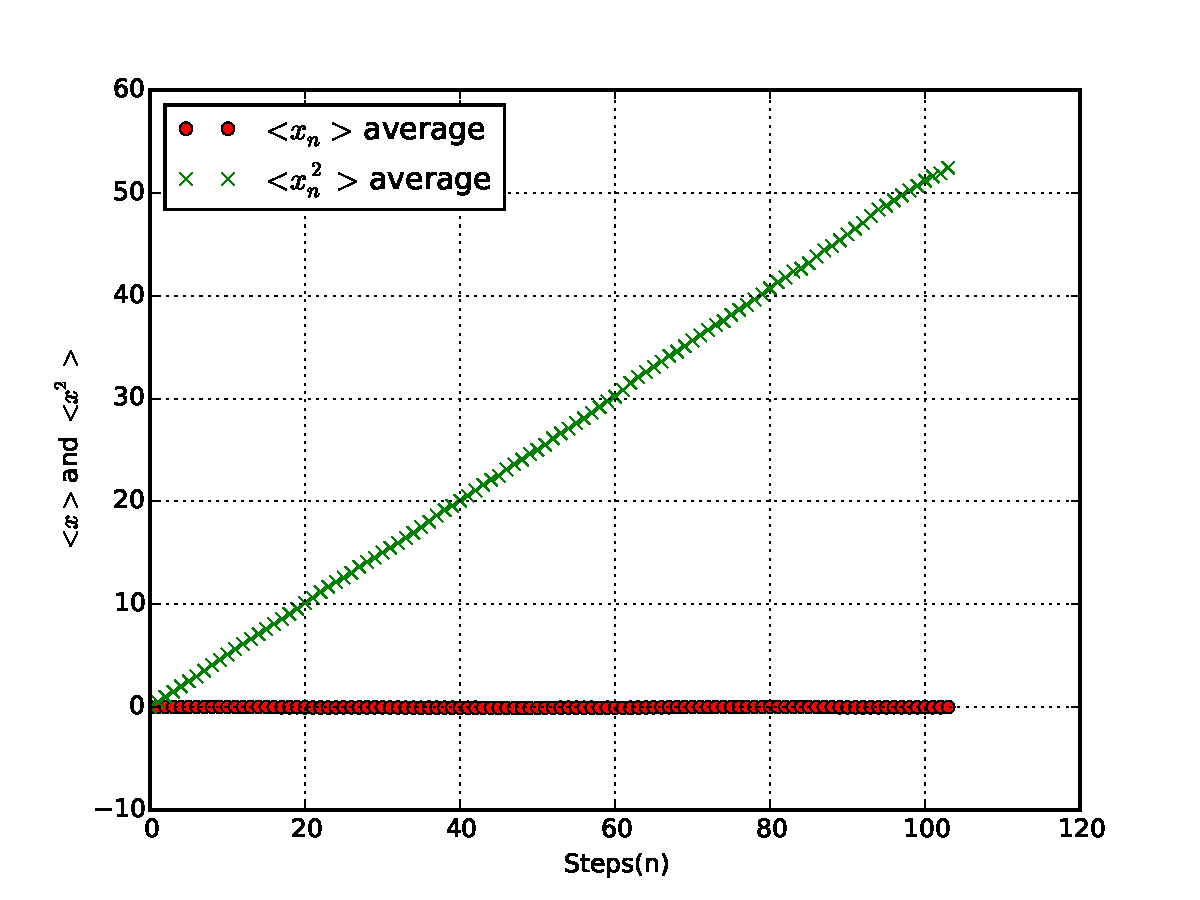
\includegraphics[width=0.8\textwidth]{rwxn.pdf}
			\caption{$ <x(t)> $ and  $ <x^2(t)> $ in 1D random walking, averaging over a 10000 random walker ensemble.}
		\end{figure}
			\begin{figure}[H]
				\centering
				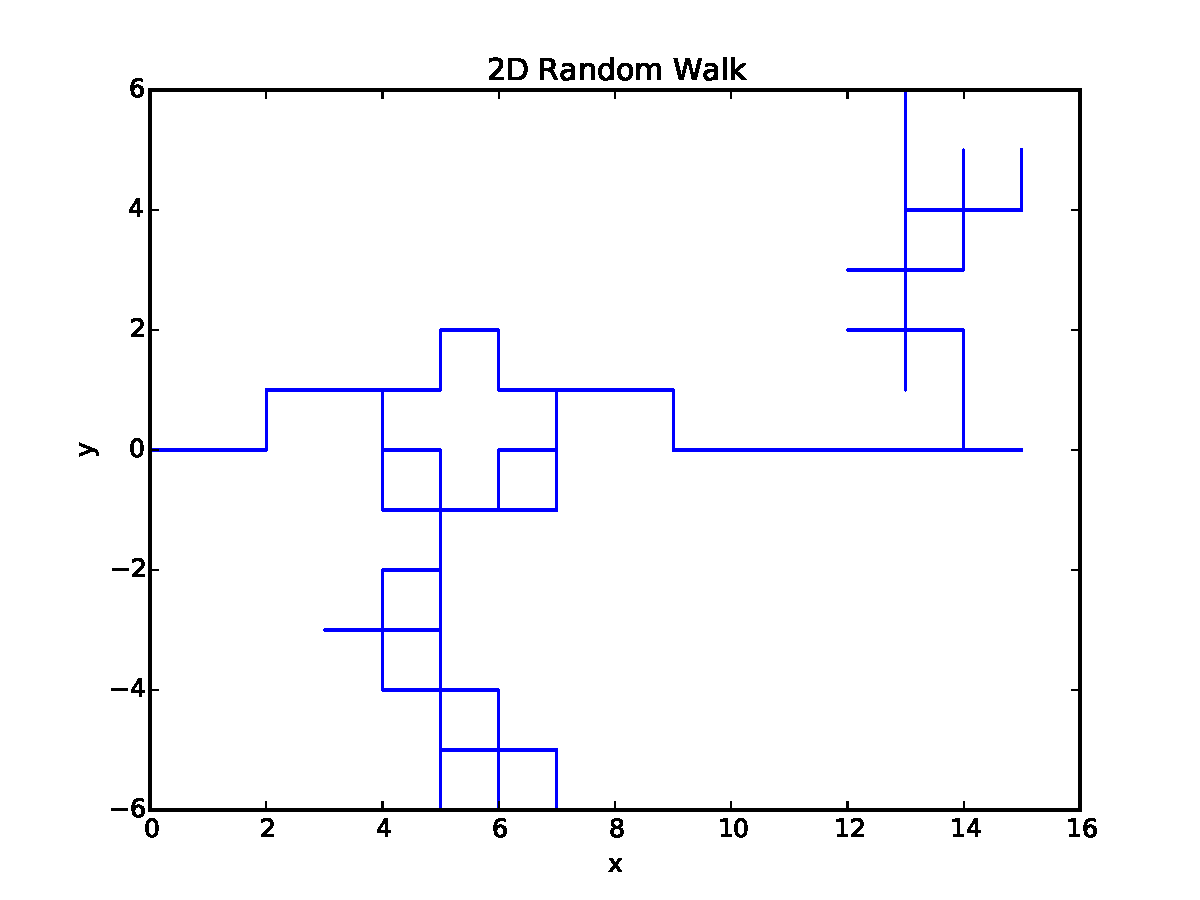
\includegraphics[width=0.8\textwidth]{rwxn3.pdf}
				\caption{A tipical 2D random walking pattern, starting from (0,0).}
			\end{figure}
		\begin{figure}[H]
			\centering
			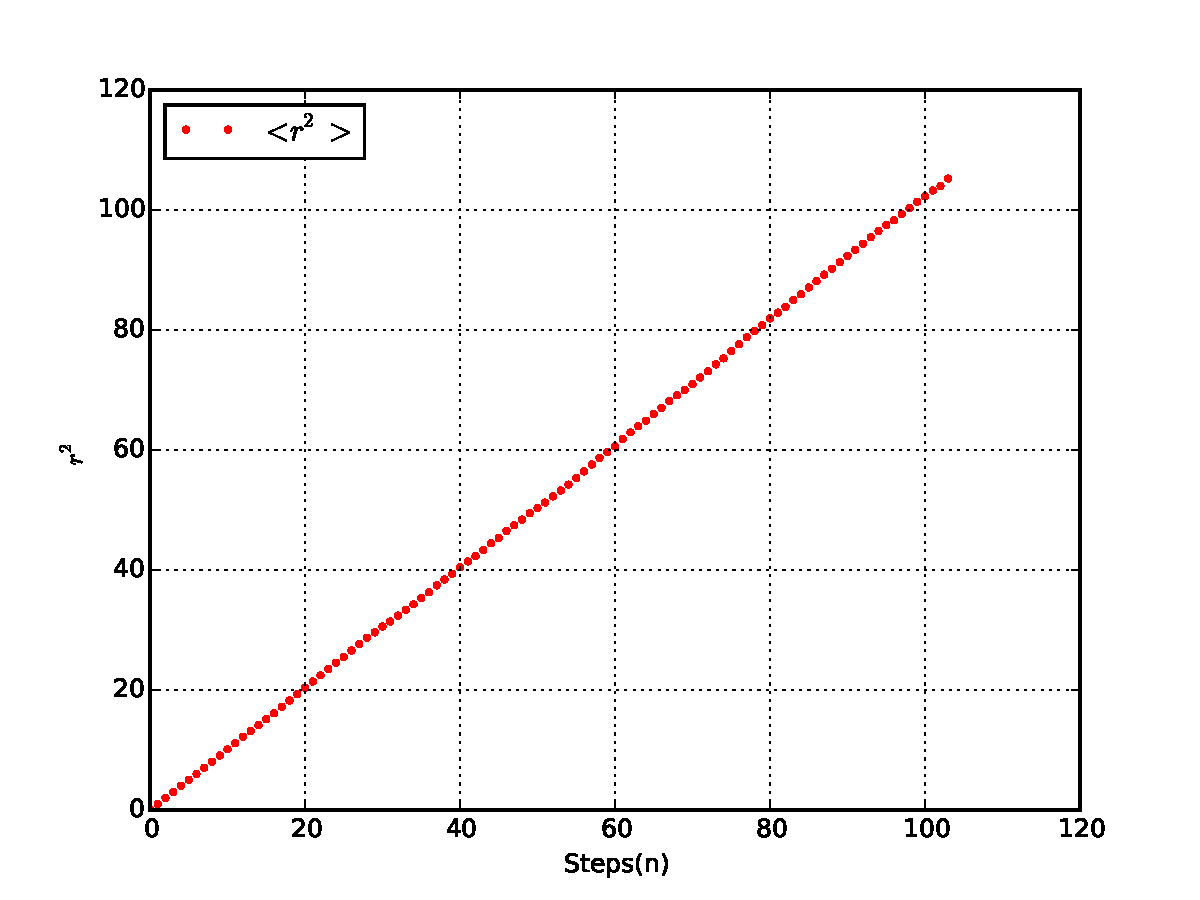
\includegraphics[width=0.8\textwidth]{rwxn2.pdf}
			\caption{$<r^2(t)>$ in 2D random walking, averaging over a 10000 random walker ensemble.}
		\end{figure}
		

	
	\section{2. Diffusion Equation}
	In this problem we aim to simulate the diffusion of one substance in another (sugar in water for instance). Diffusion will start from a box profile with a peak at origin and 10 grid around and diffuse in 1 dimension. We will found out the diffusion will approximate Gaussian distribution at later times and fit will be preformed to verify that $\sigma=\sqrt{2Dt}$ for several snapshot t.

\begin{enumerate}
\item First of all we will show analytically that the spatial expectation $\langle x(t)^2\rangle$ of the 1D normal distribution 
\begin{equation}
\rho_{(x,t)}=\frac{1}{\sqrt{2\pi}\sigma{(t)}}\exp(-\frac{x^2}{2\sigma{(t)}^2})
\end{equation}
is just $\sigma(t)^2$.

The spatial expectation
\begin{equation}
\begin{split}
\langle x(t)^2\rangle&=\int_{-\infty}^{\infty}\frac{1}{\sqrt{2\pi}\sigma(t)}x^2\exp(-\frac{x^2}{2\sigma(t)^2})dx\\
&=\frac{1}{\sqrt{2\pi}\sigma(t)}\int_{-\infty}^{\infty}x^2\exp(-\frac{x^2}{2\sigma(t)^2})dx\\
&=\frac{1}{\sqrt{2\pi}\sigma(t)}\times \sqrt{2\pi}\sigma(t)^3\\
&=\sigma(t)^2.
\end{split}
\end{equation}

So $\langle x(t)^2\rangle=\sigma(t)^2$.
\item We know the diffusion equation
\begin{equation}
\frac{\partial\rho}{\partial t}=D\nabla^2\rho
\end{equation}
If we discretize time and position to $t=k\Delta t, x=i\Delta x$, we can get the recursion equation with time, 
\begin{equation}
\rho_{i,k+1}=\rho_{i,k}+D\frac{\Delta t}{\Delta x^2}(\rho_{i+1,k}+\rho_{i-1,k}-2\rho_{i,k})
\end{equation}
here we used $\Delta t=0.002s, \Delta x=0.1m, D=2$. The relation $\Delta t<\frac{\Delta x^2}{2D}$ is satisfied to guarantee convergence.

\end{enumerate}

Then, with the initial distribution given, all future state can be solved. We here will solve the equation for 150s and take snapshot at 30s, 60s, 90s, 120s and 150s. Gaussian fit is applied to these snapshot to verify $\sigma=\sqrt{2Dt}$. Plots for the 5 snapshots and fitted Gaussian are shown in Fig. \ref{fig:diffusion1}.
\begin{figure}[H]
\centering
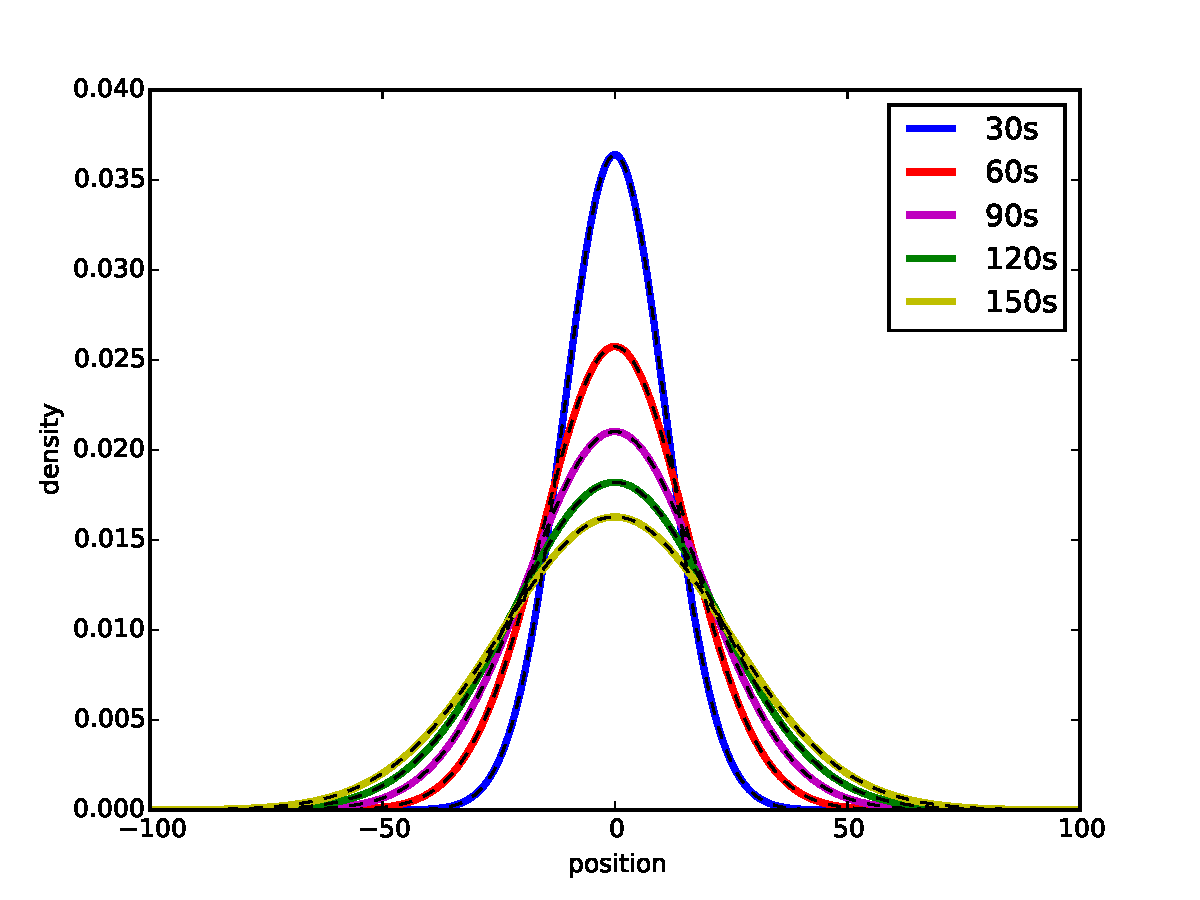
\includegraphics[width=1.0\textwidth]{diffusion.pdf}
\caption{Snapshots at 30s, 60s, 90s, 120s, 150s and comparison with fitted curve}
\label{fig:diffusion1}
\end{figure}
As for the Gaussian fit, we used the function curve\_fit from scipy.optimize. We first define the Gaussian function with input of $x, \mu, \sigma$ and call it in the function \_fit to get the optimized $\sigma$ the comparison of $\sigma$ with $\sqrt{2Dt}$ are shown in Fig. \ref{fig:diffusion2}.
\begin{figure}[H]
\centering
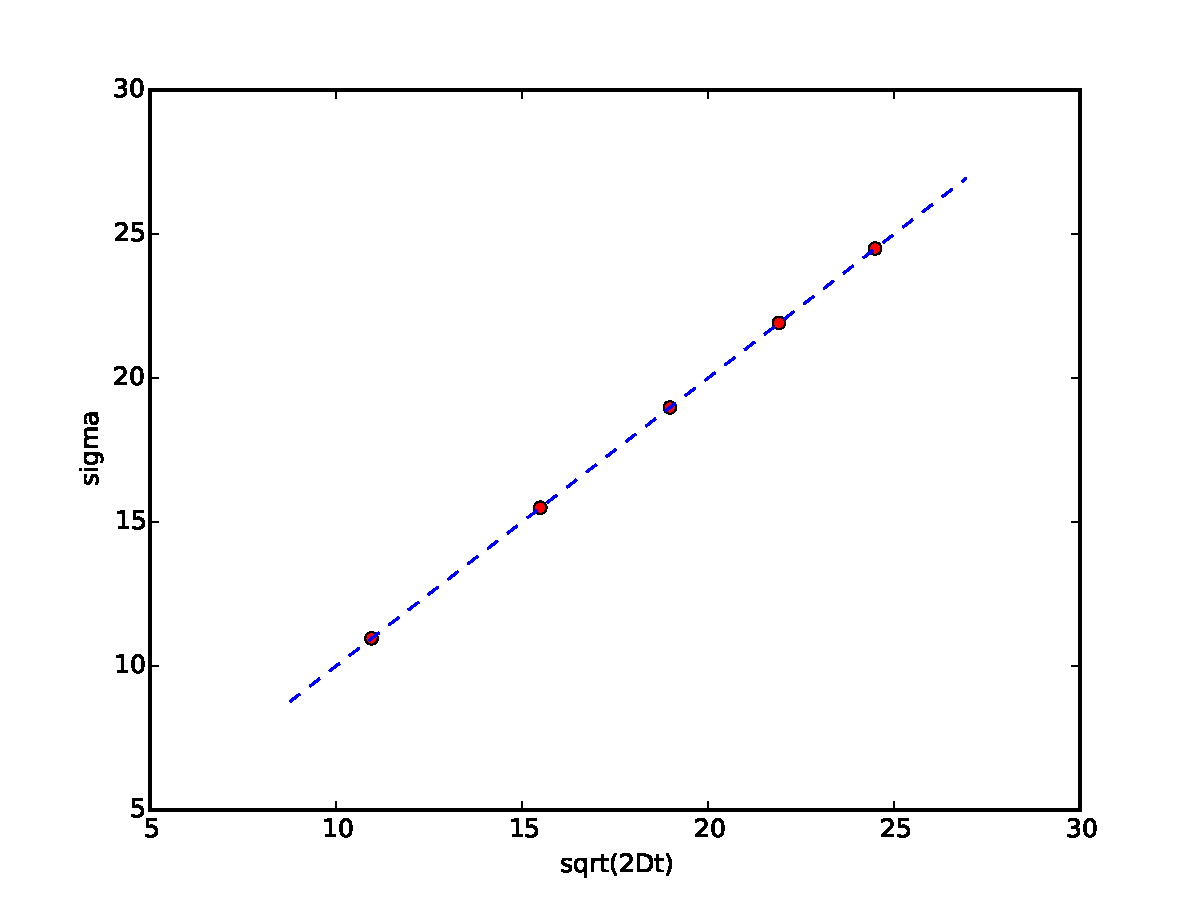
\includegraphics[width=1.0\textwidth]{sigma.pdf}
\caption{Comparison of $\sigma$ and $\sqrt{2Dt}$, the blue dashed line is $y=x$.}\label{fig:diffusion2}
\end{figure}

Thus we have used the diffusion equation to simulate the diffusion of a initial distribution of a peak (spread out a few grid) and we find that the distribution tend to approximate Gaussian distribution. We also find that the spatial spread expectation $\langle x(t)^2\rangle=2Dt$ increases linearly with time.

	\section{3. Cluster Growth with the DLA model}

Diffusion-limited aggregation (DLA) is the process whereby particles undergoing a random walk due to Brownian motion cluster together to form aggregates of such particles. This theory, proposed by T.A. Witten Jr. and L.M. Sander in 1981, is applicable to aggregation in any system where diffusion is the primary means of transport in the system. DLA can be observed in many systems such as electrodeposition, Hele-Shaw flow, mineral deposits, and dielectric breakdown.

The implementation of DLA using Python involves the following steps:\\
1. consider a lattice of points;\\
2. start with a seed particle at origin;\\
3. release a particle at a randomly chosen location some distance (here we choose 100 units) from the cluster, let it perform a random walk;\\
4. judge: if the particle stray too far away from the original, it is thrown away; if the particle reaches a perimeter site (i.e., all the unoccupied sites that are nearest neighbor to occupied sites), it becomes part of cluster;\\
5. repeat 3-4 until the cluster reaches the desired size.\\

Typical clusters grown using DLA method are very sparse, i.e., they contain many open spaces and have very irregular perimeters, as can be seen in Fig.~\ref{cluster} and~\ref{more_clusters}. 

\begin{figure}[H]
	\centering
	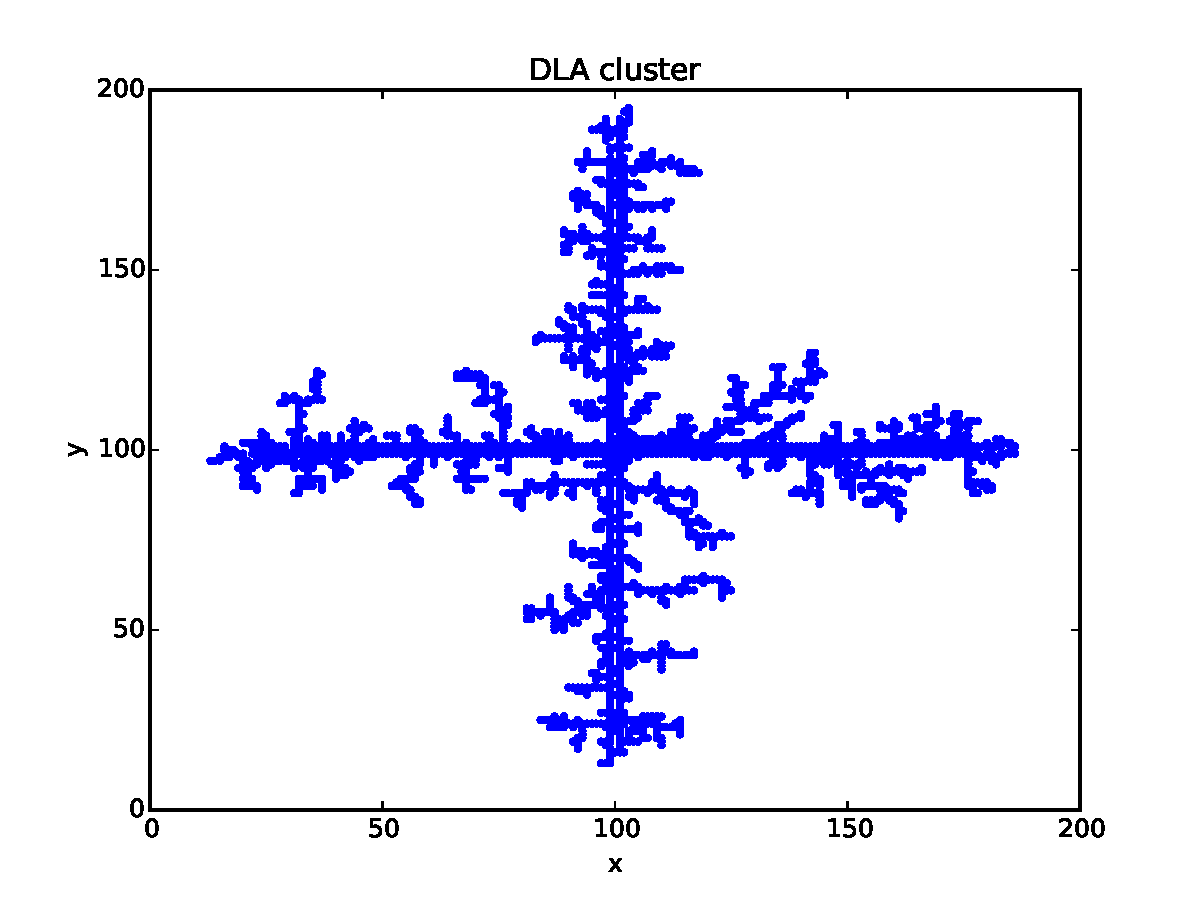
\includegraphics[width=0.8\textwidth]{dla.pdf}
	\caption{Cluster grown using DLA method. }
	\label{cluster}
\end{figure}

\begin{figure}[H]
	\centering
	\subfloat{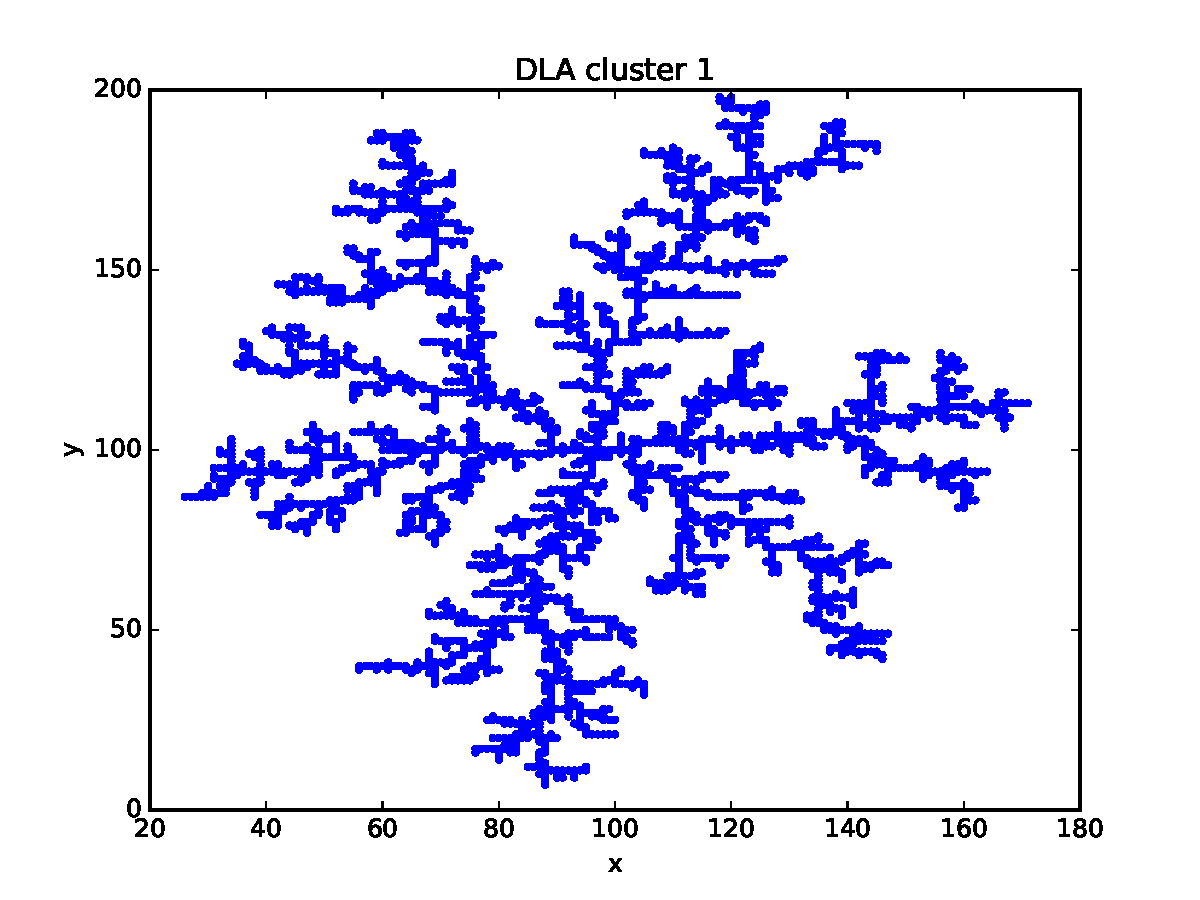
\includegraphics[width = 0.5\textwidth]{dla_0}}
	\subfloat{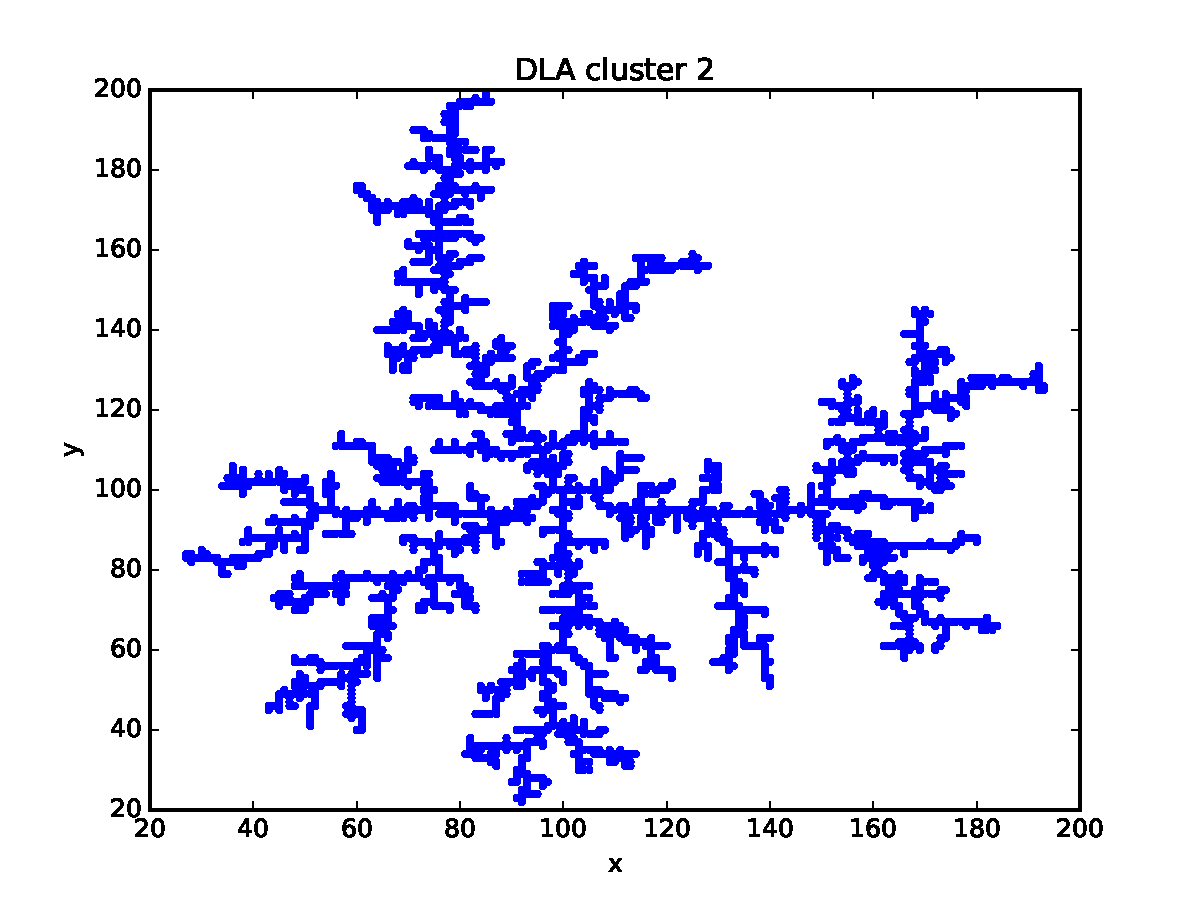
\includegraphics[width = 0.5\textwidth]{dla_1}}\\
	\subfloat{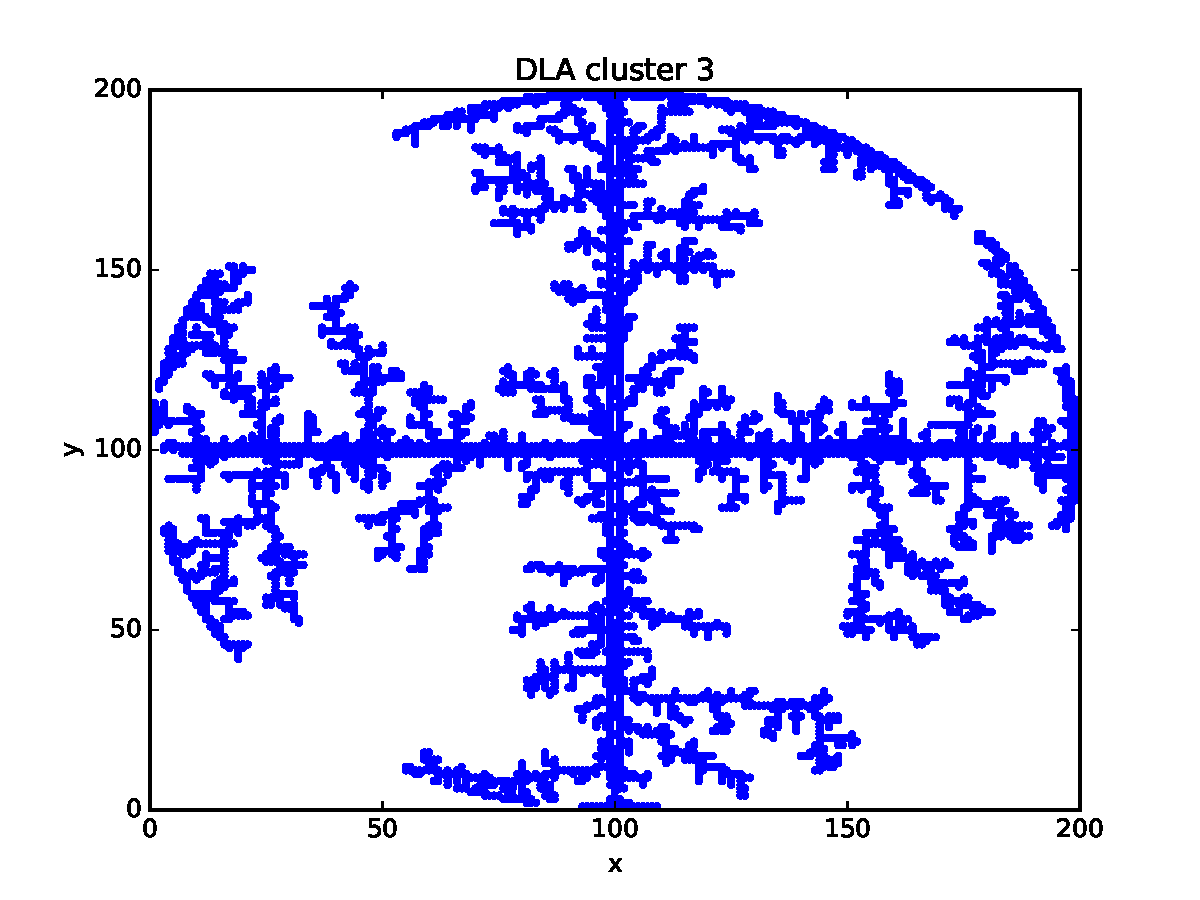
\includegraphics[width = 0.5\textwidth]{dla_2}}
	\subfloat{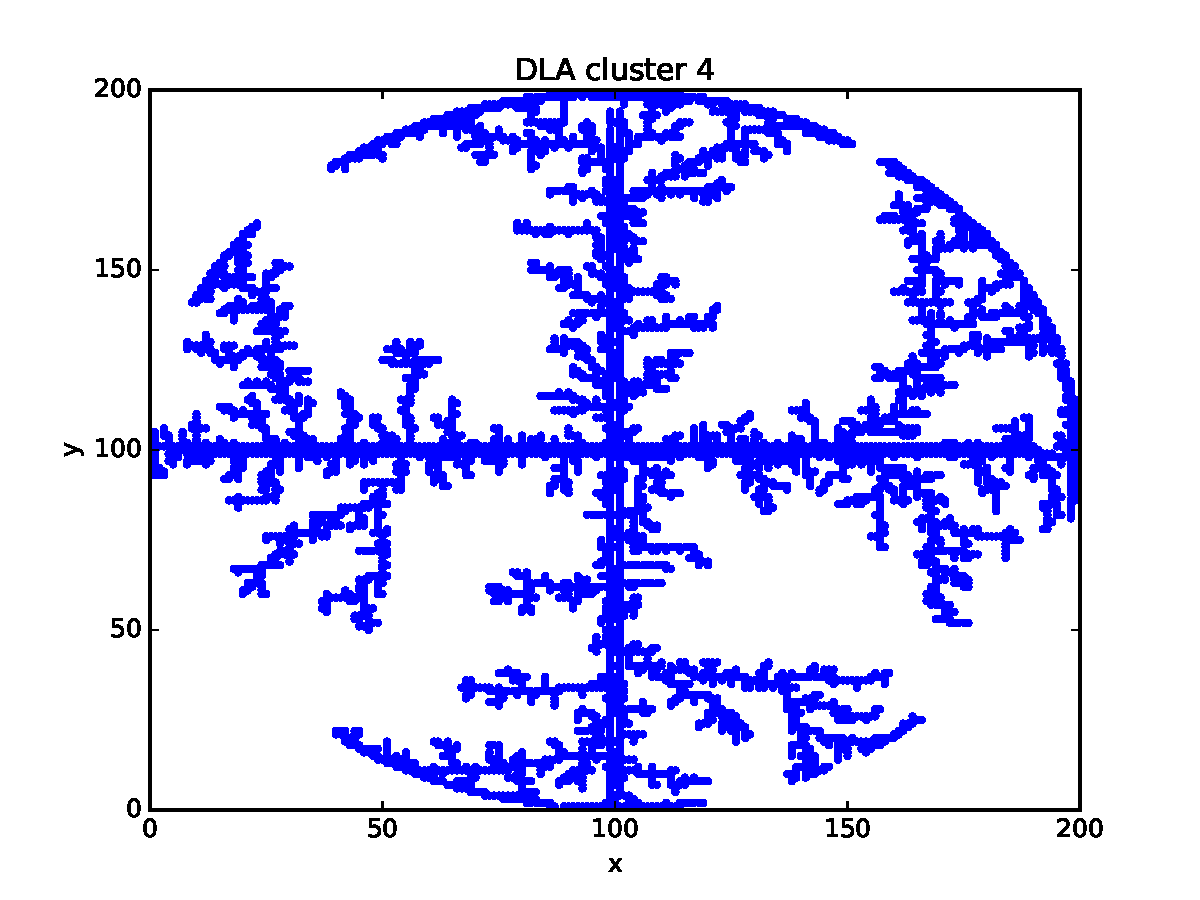
\includegraphics[width = 0.5\textwidth]{dla_3}}
	\caption{Other typical clusters grown using the DLA method}
	\label{more_clusters} 
\end{figure}


We may quantify how sparse these clusters are by considering their fractal dimension, which may be extracted by plotting the ``mass'' (how many points a cluster contains) as a function of its radius. The fractal dimensionality $d_f$ is defined as:
\begin{equation}
m(r) \sim r^{d_f}
\end{equation}
In the 2D case, the largest dimensionality comes from the most compact geometry---a uniform disk: $d_f(\text{disk}) = 2$. A line, by comparison, has $d_f(\text{line}) = 1$. The $d_f$ for DLA cluster will fall in between the two. By counting the points inside various radii $r$, then determining the slope of $\text{log}(r)\text{ vs. }\text{log}(m)$ graph, one can calculate the value of $d_f$.
\begin{equation}
\frac{\text{log}(m) }{\text{log}(r)} \sim d_f
\end{equation}
 This procedure is illustrated in Fig.~\ref{df}. In order to obtain an accurate $d_f$ value, we calculated $d_f$ for 10 distinct DLA clusters and averaged the results. These results are shown in Table~\ref{df_table}. From these results we calculate $d_f =1.68\pm 0.7$, which is in excellent agreement with the literature value of $d_f = 1.65$.
\begin{figure}[H]
	\centering
	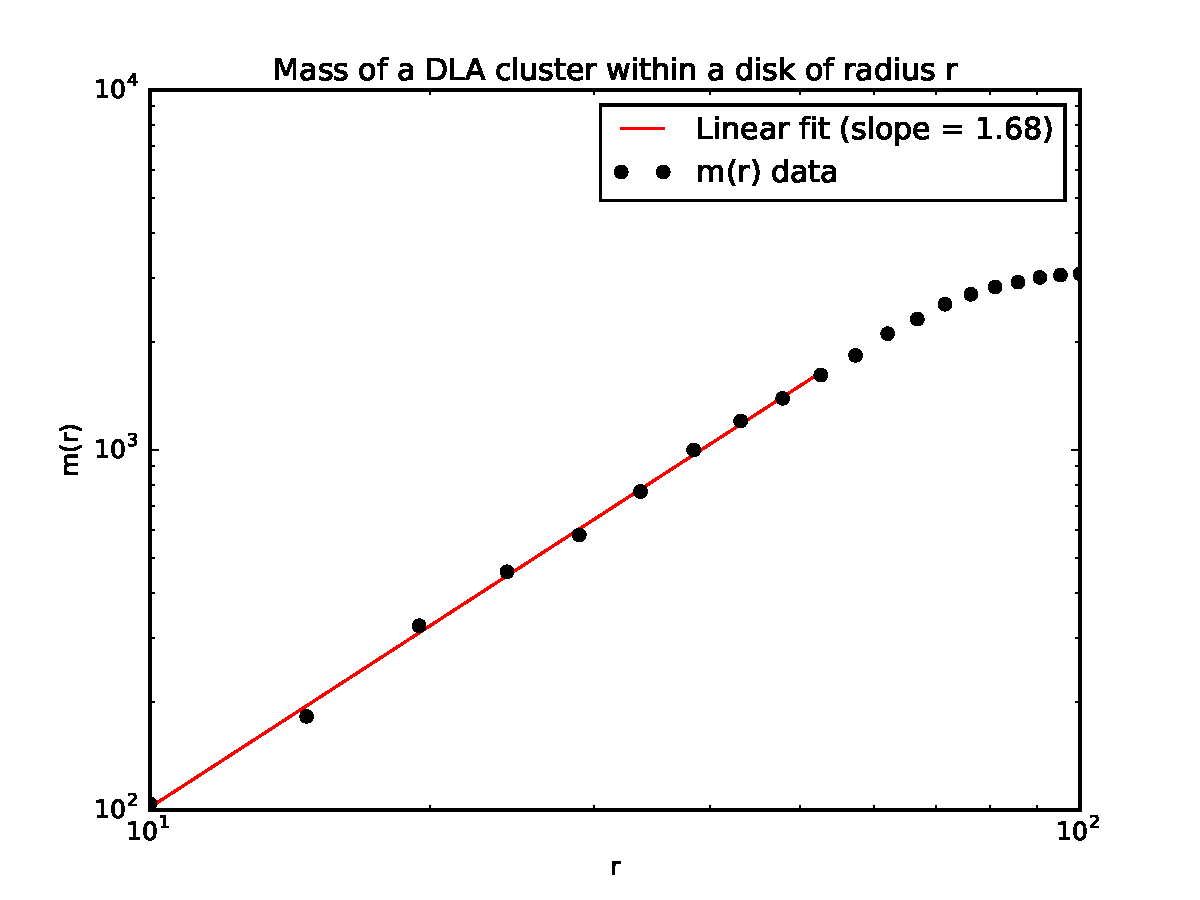
\includegraphics[width=0.8\textwidth]{mass_vs_R.pdf}
	\caption{Extraction of $d_f$ from the relation of the cluster ``mass'' and radius.}
	\label{df}
\end{figure}

\begin{table}[H]
\caption{Computed $d_f$ values for 10 different DLA clusters}
\label{df_table}
\begin{center}
\begin{tabular}{ |c|c|c|c|c|c|c|c|c|c|c| } 
 \hline
Cluster & 1 & 2 & 3 & 4 & 5 & 6 & 7 & 8 & 9 & 10 \\ 
\hline
 $d_f$& 1.74 & 1.63 & 1.77 & 1.55 & 1.66 & 1.58 & 1.64 & 1.74 & 1.74 & 1.75 \\ 
 \hline
\end{tabular}
\end{center}
\end{table}
 
 
 \section{Conclusion}
 
The above sections demonstrate the incredible versatility of stochastic algorithms; one can write algorithms to model random walks and diffusion processes, allowing one to obtain numerical estimates for quantities like the diffusion constant $D$. The estimates that we obtain via our algorithms are in excellent agreement with what may be predicted from the mathematical theory. 

The ideas and insights gained from our modeling of random walks and diffusion were then used to model cluster growth using the DLA method, which has a variety of physical analogs. Using the numerical results we were able to determine the fractal dimensionality of the DLA clusters with relative ease---determining $d_f$ analytically is certainly a much more daunting task. Thus, stochastic algorithms hold an incredibly important place in modern research, for they allow us to probe systems that may be analytically intractable.
 
\end{document}
	
	%
	% ****** End of file apssamp.tex ******
